\documentclass[aps,superscriptaddress,floatfix,nofootinbib,showpacs,amsmath,amssymb,altaffilletter,floatfix,linenumbers]{revtex4-1}
%---
%--- Packages
\usepackage[colorlinks=true,pdfstartview=FitV,linkcolor=blue,citecolor=blue,urlcolor=blue]{hyperref}
\usepackage[separate-uncertainty,retain-explicit-plus,per-mode=symbol,binary-units]{siunitx}
\usepackage{array,mathtools,amssymb,dcolumn}
\usepackage{amsmath}
\usepackage[below]{placeins}
\usepackage[table]{xcolor}
\usepackage{tikz}
\usepackage{afterpage}
\usepackage{lineno}
\usepackage{paralist}
\usepackage{listings}
\usepackage{array}
\usepackage[version=4]{mhchem}
\usepackage{multirow}
\usepackage{eurosym}
\usepackage{pagecolor}
\usepackage{fancyhdr}
%--- 1 inch margins
\usepackage{calc}
\setlength\textwidth{6.5in}
\setlength\textheight{9in}
\setlength\oddsidemargin{(\paperwidth-\textwidth)/2 - 1in} 
\setlength\evensidemargin{(\paperwidth-\textwidth)/2 - 1in} 
\setlength\topmargin{(\paperheight-\textheight-\headheight-\headsep-\footskip)/2 - 1in}
%--- Language
\lstset{language=C++,basicstyle=\ttfamily}
%--- Floats Placement
\setlength\textfloatsep{5pt}
\setlength\abovecaptionskip{5pt}
%--- Counters
\newcounter{mylistcounter}
%--- Text and References
\newcommand{\myrefs}[2]{\href{http://dx.doi.org/#2}{#1}}
\newcommand{\mref}[1]{\href{http://#1}{#1}}
\newcommand{\elog}[1]{\href{https://blackhole.lngs.infn.it/DS-50kg/#1}{#1}}
\newcommand{\mrefsec}[1]{\href{https://#1}{#1}}
\newcommand{\mrefs}[2]{\href{http://#2}{#1}}
\newcommand{\arxiv}[1]{\href{http://arxiv.org/abs/#1}{arxiv:#1}}
\newcommand{\grant}[2]{#1-#2}
\newcommand{\docdb}[1]{\href{http://darkside-docdb.fnal.gov:8080/cgi-bin/ShowDocument?docid=#1}{DarkSide DocDB \##1}}
\newcommand{\cmt}[2]{\indent{\tt \color{blue}#1: \color{red}#2}}
\newcommand{\chk}[1]{{\tt \color{red}To be checked:~#1}}
\newcommand{\fchk}[1]{{\tt \color{red}Figure to be replaced:~#1}}
\newcommand{\event}[2]{{\tt Event\# #1, Run\# #2}}
\newcommand{\minitab}[3]{\begin{tabular}{@{}#1@{}}{#2}\\{#3}\end{tabular}}
%--- Software Packages
\newcommand{\FLUKA}{\mbox{FLUKA}}
\newcommand{\Geant}{\mbox{Geant4}}
\newcommand{\GFDS}{\mbox{G4DS}}
\newcommand{\SOURCES}{\mbox{SOURCES4A}}
\newcommand{\TALYS}{\mbox{TALYS}}
\newcommand{\SRIM}{\mbox{SRIM}}
\newcommand{\LabVIEW}{\mbox{NI LabVIEW}}
\newcommand{\CERNRoot}{\mbox{Root}}
%--- Functions
\newcommand{\logten}{\ensuremath{\log_{10}}}
%--- Units
\DeclareSIUnit\c{\mbox{$c$}}
\DeclareSIUnit\magn{\mbox{$\times$}}
\DeclareSIUnit\min{min}
\DeclareSIUnit\week{week}
\DeclareSIUnit\year{yr}
\DeclareSIUnit\years{years}
\DeclareSIUnit\yr{yr}
\DeclareSIUnit\standard{std}
\DeclareSIUnit\str{sr}
\DeclareSIUnit\ppm{ppm}
\DeclareSIUnit\ppb{ppb}
\DeclareSIUnit\ppt{ppt}
\DeclareSIUnit\pe{PE}
\DeclareSIUnit\spe{SPE}
\DeclareSIUnit\ev{events}
\DeclareSIUnit\ct{counts}
\DeclareSIUnit\neutron{\mbox{$n$}}
\DeclareSIUnit\smp{samples}
\DeclareSIUnit\Sample{S}
\DeclareSIUnit\ch{ch}
\DeclareSIUnit\hit{hit}
\DeclareSIUnit\hits{hits}
\DeclareSIUnit\bin{(\mbox{5-PE}~bin)}
\DeclareSIUnit\sgm{\mbox{$\sigma$}}
\DeclareSIUnit\rms{RMS}
\DeclareSIUnit\keVr{\mbox{keV$_{\rm nr}$}}
\DeclareSIUnit\keVee{\mbox{keV$_{e{\rm e}}$}}
\DeclareSIUnit\ph{photons}
\DeclareSIUnit\pm{PMT}
\DeclareSIUnit\inch{''}
\DeclareSIUnit\bit{bit}
\DeclareSIUnit\sample{samples}
\DeclareSIUnit\barn{barn}
\DeclareSIUnit\bara{bar}
\DeclareSIUnit\barg{barg}
\DeclareSIUnit\mlardepth{\mbox(meter~of~\LAr~depth)}
\DeclareSIUnit\Curie{Ci}
\DeclareSIUnit\psi{psi}
\DeclareSIUnit\parsec{pc}
\DeclareSIUnit\liveday{\mbox{live-days}}
\DeclareSIUnit\days{\mbox{days}}
\DeclareSIUnit\day{\mbox{day}}
\DeclareSIUnit\miles{\mbox{miles}}
\DeclareSIUnit\degreeC{\mbox{$^{\circ}$C}}
\DeclareSIUnit\electron{\mbox{$e^-$}}
\DeclareSIUnit\Euro{\mbox{\euro}}
\DeclareSIUnit\cph{cph}
\DeclareSIUnit\neq{neq}
%--- Energies, Branching Ratios, and Abundances
\newcommand{\BR}{\mbox{BR}}
\newcommand{\EC}{\mbox{EC}}
\newcommand{\PositronAnnihilationGammaEnergy}{\SI{511}{\keV}}
\newcommand{\PbXRayEnergy}{\SI{46}{\keV}}
\newcommand{\HOneNeutronCaptureGammaEnergy}{\SI{2.2}{\MeV}}
\newcommand{\LiSixNaturalAbundance}{\SI{7.5}{\percent}}
\newcommand{\LiSixNeutronCaptureCrossSection}{\SI{941}{\barn}}
\newcommand{\LiSixNeutronCaptureTritonEnergy}{\SI{2.73}{\MeV}}
\newcommand{\LiSixNeutronCaptureAlphaEnergy}{\SI{2.05}{\MeV}}
\newcommand{\LiSixNeutronCaptureTritonAlphaQuenchedEnergy}{\SIrange[range-units=single]{400}{500}{\keVee}}
\newcommand{\BTenNaturalAbundance}{\SI{20}{\percent}}
\newcommand{\BTenNeutronCaptureCrossSection}{\SI{3840}{\barn}}
\newcommand{\BTenNeutronCaptureGroundDecayBR}{\SI{6.4}{\percent}}
\newcommand{\BTenNeutronCaptureGroundDecayAlphaEnergy}{\SI{1775}{\keV}}
\newcommand{\BTenNeutronCaptureExcitedDecayBR}{\SI{93.6}{\percent}}
\newcommand{\BTenNeutronCaptureExcitedDecayGammaEnergy}{\SI{478}{\keV}}
\newcommand{\BTenNeutronCaptureExcitedDecayAlphaEnergy}{\SI{1471}{\keV}}
\newcommand{\BTenNeutronCaptureExcitedDecayAlphaQuenchedEnergy}{\SIrange[range-units=single]{30}{35}{\keVee}}
\newcommand{\BTenNeutronCaptureExcitedDecayAlphaPE}{\SIrange[range-units=single]{25}{35}{\pe}}
\newcommand{\COneFourQValue}{\SI{156}{\keV}}
\newcommand{\CoFiveSevenQValue}{\SI{122}{\keV}}
\newcommand{\BaOneThreeThreeQValue}{\SI{356}{\keV}}
\newcommand{\CsOneThreeSevenQValue}{\SI{662}{\keV}}
\newcommand{\ArThreeSevenDecay}{\EC}
\newcommand{\ArThreeSevenBR}{\SI{100}{\percent}}
\newcommand{\ArThreeSevenQValue}{\SI{2.7}{\keV}}
\newcommand{\ArThreeSevenMeanLife}{\SI{50.51(3)}{\day}}
\newcommand{\ArThreeSevenHalfLife}{\SI{35.04}{\day}}
\newcommand{\ArThreeSevenKOneBR}{\SI{81.5}{\percent}}
\newcommand{\ArThreeSevenKTwoToFourBR}{\SI{8.7}{\percent}}
\newcommand{\ArThreeSevenKCaptureXRaysEnergy}{\SI{2.82}{\keV}}
\newcommand{\ArThreeNineQValue}{\SI{565}{\keV}}
\newcommand{\ArThreeNineMeanLife}{\SI{388}{\year}}
\newcommand{\RbEightThreeMeanLife}{\SI{124.4}{\day}}
\newcommand{\RbEightFiveMGammaEnergy}{\SI{514}{\keV}}
\newcommand{\RbEightFiveMMeanLife}{\SI{1.464}{\micro\s}}
\newcommand{\KrEightThreeQValue}{\SI{41.5}{\keV}}
\newcommand{\KrEightThreeMOneMeanLife}{\SI{2.64}{\hour}}
\newcommand{\KrEightThreeMOneECEnergy}{\SI{32.1}{\keV}}
\newcommand{\KrEightThreeMTwoMeanLife}{\SI{222}{\nano\second}}
\newcommand{\KrEightThreeMTwoECEnergy}{\SI{9.4}{\keV}}
\newcommand{\KrEightThreeMOneTwoECEnergy}{\SI{41.5}{\keV}}
\newcommand{\KrEightFiveGroundDecayQValue}{\SI{687}{\keV}}
\newcommand{\KrEightFiveExcitedDecayBR}{\SI{0.43}{\percent}}
\newcommand{\KrEightFiveExcitedDecayQValue}{\SI{173}{\keV}}
\newcommand{\GdNatNeutronCaptureCrossSection}{\SI{48890}{\barn}}
\newcommand{\PbTwoOneZeroHalfLife}{\SI{22.3}{\yr}}
\newcommand{\PbTwoOneZeroMeanLife}{\SI{32.0}{\yr}}
\newcommand{\PoTwoOneZeroAlphaEnergy}{\SI{5.3}{\MeV}}
\newcommand{\PoTwoOneTwoAlphaEnergy}{\SI{8.78}{\MeV}}
\newcommand{\BiTwoOneTwoAlphaOneEnergy}{\SI{6.09}{\MeV}}
\newcommand{\BiTwoOneTwoAlphaTwoEnergy}{\SI{6.05}{\MeV}}
\newcommand{\BiTwoOneTwoHalfLife}{\SI{10.6}{\hour}}
\newcommand{\PoTwoOneSixAlphaEnergy}{\SI{6.78}{\MeV}}
\newcommand{\RnTwoTwoZeroHalfLife}{\SI{56}{\second}}
\newcommand{\RnTwoTwoZeroAlphaEnergy}{\SI{6.29}{\MeV}}
\newcommand{\RnTwoTwoTwoHalfLife}{\SI{3.8}{\day}}
\newcommand{\RaTwoTwoFourHalfLife}{\SI{3.6}{\day}}
\newcommand{\ThTwoTwoEightHalfLife}{\SI{1.9}{\yr}}
\newcommand{\AmTwoFourGammaOneEnergy}{\SI{59.5}{\keV}}
\newcommand{\AmTwoFourOneGammaTwoBR}{\SI{56}{\percent}}
\newcommand{\AmBeGammaEnergy}{\SI{4.4}{\MeV}}
\newcommand{\AmBe}{\ce{^241AmBe}}
\newcommand{\AmC}{\ce{^241Am^13C}}
\newcommand{\AmCNeutronEnergy}{\SI{4}{\MeV}}
\newcommand{\DD}{\ce{^2D}-\ce{^2D}}
\newcommand{\DDNeutronEnergy}{\SI{2.45}{\MeV}}
\newcommand{\AArArThreeNineOverArFourZeroRatio}{\num{8E-16}}
\newcommand{\AArArThreeNineActivity}{\SI{1}{\becquerel\per\kg}}
\newcommand{\NeutronsPerChainDecayUTh}{\numrange{E-5}{E-7}}
\newcommand{\LArRadiogenicNeutronInteractionLength}{\SI{~10}{\cm}}
%--- Cosmology
\newcommand{\LCDM}{\mbox{$\Lambda$CDM}}
%--- Solar Neutrinos
\newcommand{\PP}{\mbox{$pp$}}
\newcommand{\PEP}{\mbox{$pep$}}
\newcommand{\CNO}{\mbox{CNO}}
%--- Names
\newcommand{\DS}{\mbox{DarkSide}}
\newcommand{\DSt}{\mbox{DarkSide-10}}
\newcommand{\DSf}{\mbox{DarkSide-50}}
\newcommand{\DSp}{\mbox{DarkSide-Proto}}
\newcommand{\DSk}{\mbox{DarkSide-20k}}
\newcommand{\DSs}{\mbox{DS}}
\newcommand{\DSts}{\mbox{DS-10}}
\newcommand{\DSfs}{\mbox{DS-50}}
\newcommand{\DSps}{\mbox{DS-Proto}}
\newcommand{\DSks}{\mbox{DS-20k}}
\newcommand{\DSCollaborators}{\num{\sim~300}}
\newcommand{\DSInstitutes}{\num{\sim~70}}
\newcommand{\DSCountries}{\num{15}}
\newcommand{\GADMC}{\mbox{GADMC}}
\newcommand{\DEAP}{\mbox{DEAP-3600}}
\newcommand{\mCLEAN}{\mbox{MiniCLEAN}}
\newcommand{\ArDM}{\mbox{ArDM}}
\newcommand{\Argo}{\mbox{Argo}}
\newcommand{\ThreeDPi}{\mbox{3D$\pi$}}
\newcommand{\FBP}{\mbox{FBP}}
\newcommand{\BX}{\mbox{Borexino}}
\newcommand{\SNO}{\mbox{SNO}}
\newcommand{\SCENE}{\mbox{SCENE}}
\newcommand{\ReD}{\mbox{ReD}}
\newcommand{\ARIS}{\mbox{ARIS}}
\newcommand{\Urania}{\mbox{Urania}}
\newcommand{\Aria}{\mbox{Aria}}
\newcommand{\Seruci}{\mbox{Seruci}}
\newcommand{\SeruciZero}{\mbox{Seruci-0}}
\newcommand{\SeruciOne}{\mbox{Seruci-I}}
\newcommand{\SeruciTwo}{\mbox{Seruci-II}}
\newcommand{\LOGAN}{\mbox{LOGAN}}
\newcommand{\DART}{\mbox{DART}}
\newcommand{\MAWG}{M\&A\,WG}
\newcommand{\CTF}{\mbox{CTF}}
\newcommand{\WBS}{\mbox{WBS}}
\newcommand{\CROne}{\mbox{CR1}}
\newcommand{\CRH}{\mbox{CRH}}
\newcommand{\LSV}{\mbox{LSV}}
\newcommand{\WCV}{\mbox{WCV}}
\newcommand{\wt}{\mbox{WT}}
\newcommand{\TPC}{\mbox{TPC}}
\newcommand{\TPCs}{\mbox{TPCs}}
\newcommand{\LArTPC}{\mbox{LAr~TPC}}
\newcommand{\LArTPCs}{\mbox{LAr~TPCs}}
\newcommand{\calis}{\mbox{CALIS}}
\newcommand{\UV}{\mbox{UV}}
\newcommand{\NUV}{\mbox{NUV}}
\newcommand{\TMF}{\mbox{TMF}}
\newcommand{\PMT}{\mbox{PMT}}
\newcommand{\PMTs}{\mbox{\PMT s}}
\newcommand{\MCP}{\mbox{MCP}}
\newcommand{\MCPPMT}{\mbox{\MCP-\PMT}}
\newcommand{\MCPPMTs}{\mbox{\MCPPMT s}}
\newcommand{\SiPM}{\mbox{SiPM}}
\newcommand{\SiPMs}{\mbox{SiPMs}}
\newcommand{\RGBHd}{\mbox{RGB-HD}}
\newcommand{\RGBHdSf}{\mbox{RGB-HD-SF}}
\newcommand{\RGBHdSfHRq}{\mbox{RGB-HD-HR$_q$}}
\newcommand{\RGBHdSfLRq}{\mbox{RGB-HD-LR$_q$}}
\newcommand{\NUVHd}{\mbox{NUV-HD}}
\newcommand{\NUVHdSf}{\mbox{NUV-HD-SF}}
\newcommand{\NUVHdLf}{\mbox{NUV-HD-LF}}
\newcommand{\NUVHdSfHRq}{\mbox{NUV-HD-SF-HR$_q$}}
\newcommand{\NUVHdSfLRq}{\mbox{NUV-HD-SF-LR$_q$}}
\newcommand{\NUVHdLfHRq}{\mbox{NUV-HD-LF-HR$_q$}}
\newcommand{\NUVHdLfLRq}{\mbox{NUV-HD-LF-LR$_q$}}
\newcommand{\HRq}{\mbox{HR$_q$}}
\newcommand{\LRq}{\mbox{LR$_q$}}
\newcommand{\HD}{\mbox{HD}}
\newcommand{\CTE}{\mbox{CTE}}
\newcommand{\PCB}{\mbox{PCB}}
\newcommand{\PCBs}{\mbox{PCBs}}
\newcommand{\TSV}{\mbox{TSV}}
\newcommand{\TSVs}{\mbox{TSVs}}
\newcommand{\tile}{\mbox{tile}}
\newcommand{\tiles}{\mbox{tiles}}
\newcommand{\SPAD}{\mbox{SPAD}}
\newcommand{\SPADs}{\mbox{SPADs}}
\newcommand{\QE}{\mbox{QE}}
\newcommand{\PDE}{\mbox{PDE}}
\newcommand{\OV}{\mbox{OV}}
\newcommand{\LV}{\mbox{LV}}
\newcommand{\SCR}{\mbox{SCR}}
\newcommand{\DCR}{\mbox{DCR}}
\newcommand{\DiCT}{\mbox{DiCT}}
\newcommand{\DeCT}{\mbox{DeCT}}
\newcommand{\AP}{\mbox{AP}}
\newcommand{\DLED}{\mbox{DLED}}
\newcommand{\TCNR}{\mbox{TCNR}}
\newcommand{\TCNP}{\mbox{TCNP}}
\newcommand{\CMOS}{\mbox{CMOS}}
\newcommand{\HLST}{\mbox{HLST}}
\newcommand{\SQB}{\mbox{SQB}}
\newcommand{\SQBs}{\mbox{\SQB s}}
\newcommand{\TRB}{\mbox{TRB}}
\newcommand{\TRBs}{\mbox{\TRB s}}
\newcommand{\WIMP}{\mbox{WIMP}}
\newcommand{\WIMPs}{\mbox{\WIMP s}}
\newcommand{\MC}{\mbox{MC}}
\newcommand{\DAQ}{\mbox{DAQ}}
\newcommand{\ADC}{\mbox{ADC}}
\newcommand{\ADCs}{\mbox{\ADC s}}
\newcommand{\TDC}{\mbox{TDC}}
\newcommand{\TDCs}{\mbox{\TDC s}}
\newcommand{\artdaq}{\mbox{artdaq}}
\newcommand{\TMB}{\mbox{TMB}}
\newcommand{\PC}{\mbox{PC}}
\newcommand{\PCTMB}{\mbox{\PC-\TMB}}
\newcommand{\PPO}{\mbox{PPO}}
\newcommand{\BisMSB}{\mbox{BisMSB}}
\newcommand{\POPOP}{\mbox{POPOP}}
\newcommand{\DIN}{\mbox{DIN}}
\newcommand{\LAB}{\mbox{LAB}}
\newcommand{\PXE}{\mbox{PXE}}
\newcommand{\ITO}{\mbox{ITO}}
\newcommand{\PTFE}{\mbox{PTFE}}
\newcommand{\FEP}{\mbox{FEP}}
\newcommand{\TPB}{\mbox{TPB}}
\newcommand{\og}{\mbox{Operations Group}}
\newcommand{\VUV}{\mbox{VUV}}
\newcommand{\LAr}{\ce{LAr}}
\newcommand{\GAr}{\ce{GAr}}
\newcommand{\AAr}{\ce{AAr}}
\newcommand{\UAr}{\ce{UAr}}
\newcommand{\DAr}{\ce{DAr}}
\newcommand{\LRAr}{\ce{LRAr}}
\newcommand{\LIN}{\ce{LN2}}
\newcommand{\LXe}{\ce{LXe}}
\newcommand{\HPGe}{\mbox{HPGe}}
\newcommand{\HVFT}{\mbox{HVFT}}
\newcommand{\UHMWPE}{\mbox{UHMWPE}}
\newcommand{\TOF}{\mbox{TOF}}
\newcommand{\PET}{\mbox{PET}}
\newcommand{\TOFPET}{\mbox{\TOF-\PET}}
\newcommand{\PETCT}{\mbox{\PET /CT}}
\newcommand{\FDG}{\mbox{\ce{^18F}-FDG}}
\newcommand{\LOR}{\mbox{LOR}}
\newcommand{\CPU}{\mbox{CPU}}
\newcommand{\CT}{\mbox{CT}}
\newcommand{\CPUs}{\mbox{CPUs}}
\newcommand{\STEM}{\mbox{STEM}}
\newcommand{\ROI}{\mbox{ROI}}
\newcommand{\SPE}{\mbox{SPE}}
\newcommand{\SNR}{\mbox{SNR}}
\newcommand{\SNRAmp}{\mbox{SNR$_{\rm Amplitude}$}}
\newcommand{\SNRCharge}{\mbox{SNR$_{\rm Charge}$}}
\newcommand{\SNRFast}{\mbox{SNR$_{\rm Fast}$}}
\newcommand{\SNRFilter}{\mbox{SNR$_{\rm Filtered}$}}
\newcommand{\OA}{\mbox{OA}}
\newcommand{\GBP}{\mbox{GBP}}
\newcommand{\TIA}{\mbox{TIA}}
\newcommand{\TIAs}{\mbox{\TIA s}}
\newcommand{\FEB}{\mbox{FEB}}
\newcommand{\FEBs}{\mbox{\FEB s}}
\newcommand{\VFEB}{\mbox{VFEB}}
\newcommand{\VFEBs}{\mbox{\VFEB s}}
\newcommand{\VDCB}{\mbox{VDCB}}
\newcommand{\VDCBs}{\mbox{\VDCB s}}
\newcommand{\AVol}{\mbox{$A_{\tiny\rm Vol}$}}
\newcommand{\NoG}{\mbox{NG}}
\newcommand{\NoGTrue}{\mbox{$\NoG_{\rm True}$}}
\newcommand{\Tz}{\mbox{$T_z$}}
\newcommand{\eno}{\mbox{$e_n$}}
\newcommand{\enot}{\mbox{$e_n^2$}}
\newcommand{\ino}{\mbox{$i_n$}}
\newcommand{\inot}{\mbox{$i_n^2$}}
\newcommand{\Vno}{\mbox{$V_n$}}
\newcommand{\Vnot}{\mbox{$V_n^2$}}
\newcommand{\VnoTot}{\mbox{$V_n^{\rm Tot}$}}
\newcommand{\fRes}{\mbox{$f_{\rm Res}$}}
\newcommand{\FTDb}{\mbox{$f_{\rm 3Db}$}}
\newcommand{\FSDb}{\mbox{$f_{\rm 6Db}$}}
\newcommand{\TDb}{\SI{3}{\decibel}}
\newcommand{\SDb}{\SI{6}{\decibel}}
\newcommand{\PSDno}{\mbox{$\rm PSD_{n}$}}
\newcommand{\PSDnoReferencePower}{\SI{1}{\milli\watt}}
\newcommand{\NSF}{\mbox{NSF}}
\newcommand{\RAS}{\mbox{RAS}}
\newcommand{\GSSI}{\mbox{GSSI}}
\newcommand{\INFN}{\mbox{INFN}}
\newcommand{\MIUR}{\mbox{MIUR}}
\newcommand{\CERN}{\mbox{CERN}}
\newcommand{\LHC}{\mbox{LHC}}
\newcommand{\CFI}{\mbox{CFI}}
\newcommand{\NSERC}{\mbox{NSERC}}
\newcommand{\LNGS}{\mbox{LNGS}}
\newcommand{\LSC}{\mbox{LSC}}
\newcommand{\SNOLab}{\mbox{SNOLab}}
\newcommand{\TRIUMF}{\mbox{TRIUMF}}
\newcommand{\LNS}{\mbox{LNS}}
\newcommand{\DUNE}{\mbox{DUNE}}
\newcommand{\CNAF}{\mbox{CNAF}}
\newcommand{\PoliMi}{\mbox{PoliMi}}
\newcommand{\FBKTIFPA}{\mbox{FBK/TIFPA}}
\newcommand{\FBK}{\mbox{FBK}}
\newcommand{\MPD}{\mbox{MPD}}
\newcommand{\LFoundry}{\mbox{LFoundry}}
\newcommand{\SensL}{\mbox{SensL}}
\newcommand{\NOA}{\mbox{NOA}}
\newcommand{\LSO}{\mbox{LSO}}
\newcommand{\LYSO}{\mbox{LYSO}}
\newcommand{\CRT}{\mbox{CRT}}
\newcommand{\ASIC}{\mbox{ASIC}}
\newcommand{\ASICs}{\mbox{ASICs}}
\newcommand{\PSA}{\mbox{PSA}}
\newcommand{\UHV}{UHV}
\newcommand{\HalfLife}{\mbox{$\tau_{\frac{1}{2}}$}}
\newcommand{\ICPMS}{\mbox{ICP-MS}}
\newcommand{\LA}{\mbox{LA}}
\newcommand{\LAICPMS}{\mbox{\LA-\ICPMS}}
\newcommand{\BiPo}{\mbox{BiPo-3}}
\newcommand{\PEB}{\mbox{PEB}}
\newcommand{\PEBs}{\mbox{PEBs}}
\newcommand{\VO}{\mbox{VO}}
\newcommand{\LiDaR}{\mbox{LiDaR}}
\newcommand{\ArlonFiveFiveNT}{\mbox{Arlon~55-NT}}
\newcommand{\ArlonEightFiveN}{\mbox{Arlon~85-N}}
\newcommand{\ArlonEightFiveNT}{\mbox{Arlon~85-NT}}
\newcommand{\THERMOUNT}{\mbox{THERMOUNT\textregistered RT\textsuperscript{TM}}}
\newcommand{\Vikuiti}{\mbox{3M Vikuiti\textsuperscript{TM}}}
%--- Global Symbols
\newcommand{\OmegaNonBaryonicFraction}{\num{0.85}}
\newcommand{\OmegaNonBaryonicPercent}{\SI{85}{\percent}}
\newcommand{\RhoDMSymbol}{\mbox{$\rho_{\rm dm}$}}
\newcommand{\RhoDMValue}{\SI{0.3}{\GeV\per\square\c\per\cubic\cm}}
\newcommand{\VelocityNaughtSymbol}{\mbox{$v_0$}}
\newcommand{\VelocityNaughtValue}{\SI{220}{\km\per\s}}
\newcommand{\VelocityEarthSymbol}{\mbox{$v_{\rm Earth}$}}
\newcommand{\VelocityEarthValue}{\SI{232}{\km\per\s}}
\newcommand{\VelocityEscapeSymbol}{\mbox{$v_{\rm escape}$}}
\newcommand{\VelocityEscapeValue}{\SI{544}{\km\per\s}}
\newcommand{\WIMPMassSymbol}{\mbox{m_\chi}}
\newcommand{\WIMPMassLowLimit}{\SI{50}{\GeV\per\square\c}}
\newcommand{\WIMPMassHundredGev}{\SI{100}{\GeV\per\square\c}}
\newcommand{\WIMPMassOneTev}{\SI{1}{\TeV\per\square\c}}
\newcommand{\WIMPMassTenTev}{\SI{10}{\TeV\per\square\c}}
\newcommand{\LArNormalTemperature}{\SI{87}{\kelvin}}
\newcommand{\LINNormalTemperature}{\SI{77}{\kelvin}}
\newcommand{\LXeNormalTemperature}{\SI{165}{\kelvin}}
\newcommand{\RoomTemperature}{\SI{300}{\kelvin}}
\newcommand{\ElectronMass}{\SI{511}{\keV\per\square\c}}
\newcommand{\LHCCenterOfMassEnergy}{\SI{13}{TeV}}
\newcommand{\LHCDirectSearchesWIMPMassTurnoverThreshold}{\text{a few hundred~\si{GeV\per\square\c}}}
\newcommand{\BackgroundFreeRequirement}{\SI{<0.1}{\ev}}
\newcommand{\ZeroBackgroundNinetyPerCentCLEventsLimit}{\SI{2.3}{\ev}}
\newcommand{\NinetyPerCentCL}{\mbox{\SI{90}{\percent}~C.L.}}
\newcommand{\ArScintillationYield}{\SI{4E4}{\ph\per\MeV}}
\newcommand{\ArWaveLength}{\SI{128}{\nano\meter}}
\newcommand{\TPBWaveLength}{\SI{420}{\nano\meter}}
\newcommand{\XeWaveLength}{\SI{172}{\nano\meter}}
\newcommand{\NR}{\mbox{NR}}
\newcommand{\NRs}{\mbox{NRs}}
\newcommand{\ER}{\mbox{ER}}
\newcommand{\ERs}{\mbox{ERs}}
\newcommand{\bg}{\mbox{$\beta/\gamma$}}
\newcommand{\bgs}{\mbox{$\beta/\gamma$'s}}
\newcommand{\gr}{\mbox{$\gamma$-ray}}
\newcommand{\grs}{\mbox{$\gamma$-rays}}
\newcommand{\bta}{\mbox{$\beta$}}
\newcommand{\btas}{\mbox{$\beta$'s}}
\newcommand{\LEff}{\mbox{$\mathcal{L}_{\rm eff}$}}
\newcommand{\SOne}{\mbox{S1}}
\newcommand{\STwo}{\mbox{S2}}
\newcommand{\STwoSoneRatio}{\mbox{S2/S1}}
\newcommand{\SThree}{\mbox{S3}}
\newcommand{\GWL}{\mbox{GWL}}
\newcommand{\LWL}{\mbox{LWL}}
\newcommand{\mbb}{\mbox{$m_{\beta\beta}$}}
\newcommand{\qbb}{\mbox{$Q_{\beta\beta}$}}
\newcommand{\bb}{\mbox{$\beta$$\beta$}}
\newcommand{\obb}{\mbox{0$\nu$$\beta$$\beta$}}
\newcommand{\toh}{\mbox{T$^{0\nu}_{1/2}$}}
\newcommand{\tth}{\mbox{T$^{2\nu}_{1/2}$}}
\newcommand{\aSe}{\mbox{a-\ce{Se}}}

\usepackage{fancyhdr}
\usepackage{enumitem}
%\linespread{0.9}
\fancyhf{}
\renewcommand{\headrulewidth}{0pt}
\rfoot{\thepage}
\pagestyle{fancy}
%\linespread{0}
\renewcommand{\thepage}{}
\renewcommand{\thepage}{\arabic{page}}
\renewcommand\thesection{\arabic{section}}
\renewcommand\thesubsection{\thesection.\arabic{subsection}}
%\nolinenumbers
%---
\begin{document}
%---
\title{SORA}

\begin{abstract}
\begin{center}
{\bf Abstract}
\end{center}
The SORA payload sampled for the existence of microorganisms and bacterial spores in the upper atmosphere. The payload analyzed different aspects of the surrounding environment such as radiation exposure, temperature, pressure and humidity. The payload had three main scientific objectives. First, design and build a novel system that will isolate surrounding air and sample for cells. Second, onboard sensors will analyze exposure to solar and cosmic radiation that microorganisms may encounter. Finally, monitor the environmental conditions such as temperature, pressure, and humidity. Furthermore, the design employed additive manufacturing and hobby electronics in its construction to provide an accessible basis for future missions and explore the bounds of the technology available.
\end{abstract}

\newcommand{\Houston}{Department of Physics, University of Houston, Houston, TX 77204, USA}
%--- Add other authors in the order they should appear

\author{S.~A.~Garcia~Morelos}\affiliation{\Houston}
\author{F.~Brooks}\affiliation{\Houston}
\author{S.~Oliver}\affiliation{\Houston}
\author{A.~Walker}\affiliation{\Houston}
\author{K.~Portillo}\affiliation{\Houston}
\author{R.~Masek}\affiliation{\Houston}
\author{D.~Mroczek}\affiliation{\Houston}
\author{D.~De~La~Pena}\affiliation{\Houston}
\author{J.~Juarez}\affiliation{\Houston}
\author{A.~Cruz}\affiliation{\Houston}
\author{D.~Henandez}\affiliation{\Houston}
\author{A.~L.~Renshaw}\affiliation{\Houston}





\setlength{\parindent}{1em}
\setdefaultleftmargin{1em}{1em}{}{}{}{}
%---
\setcounter{page}{0}\thispagestyle{empty}
%---
\maketitle
\tableofcontents
\setcounter{page}{0}\thispagestyle{empty}
\newpage
%---
Section: Introduction
\section{Mission Statement and Objectives}
\label{sec:Introduction}

Our goal for the HASP 2018 payload is to further build upon the first SORA~\cite{SORA} flight.  In order to confirm our findings from SORA 2017, we need to again collect extremophile bacteria that reside in the upper atmosphere at approximately 36 to 41 kilometers.  A MiniPIX particle detector will be flown onboard to further study the effects of ionizing radiation on these living organisms and other various sensors will gather data pertaining to the environmental conditions in which these extremophiles reside. Due to the limited amount of data for the 20 to 40 kilometer altitude range, we have generated questions, hypotheses and objectives, based on past HASP payloads and other high altitude collection flights, that have thus far remained unanswered or have little corroborating data.

%\begin{figure}[h!]
%  \begin{center}
%    \begin{minipage}[c]{0.45\linewidth}
%      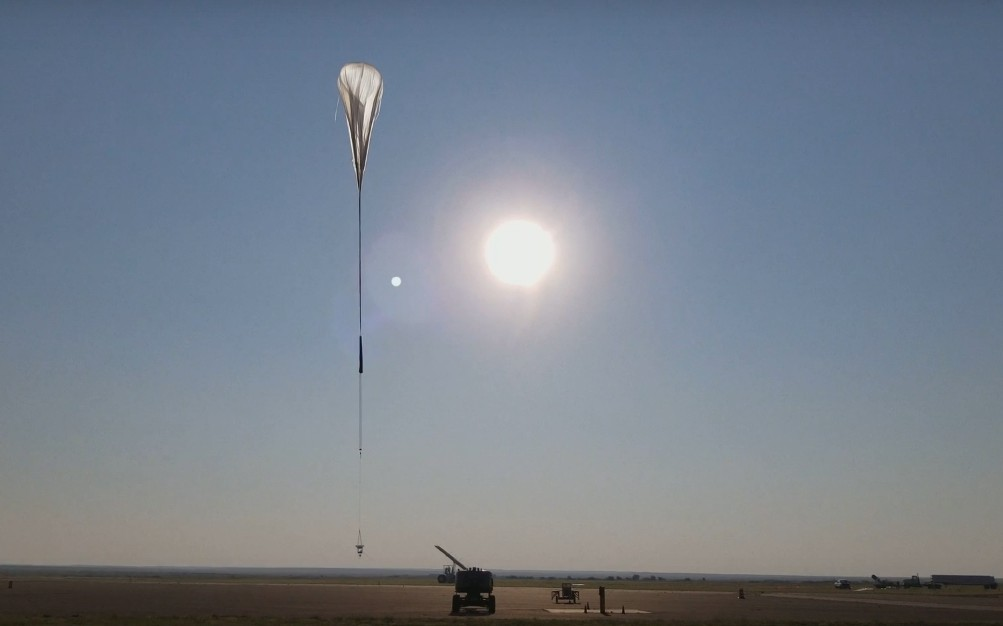
\includegraphics[width=\textwidth]{./Figures/sora_takeoff.jpg}
%      \caption{HASP platform at launch with the SORA payload onboard.}
%      \label{fig:takeoff}
%    \end{minipage}
%    \hfill
%    \begin{minipage}[c]{0.49\linewidth}
%      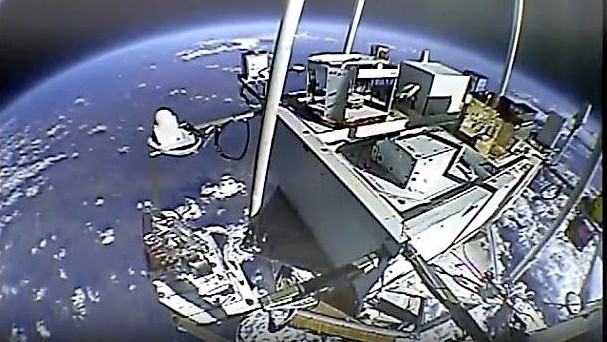
\includegraphics[width=\textwidth]{./Figures/sora_flight.jpg}
%      \caption{HASP platform at float, the SORA payload is the only gold foil covered payload onboard.}
%      \label{fig:float}
%    \end{minipage}
%  \end{center}
%\end{figure}

The main goals for SORA are to collect extremophile organisms that reside in the upper atmosphere, study the effects of surrounding radiation on these organisms in the stratosphere and gather data pertaining to the environmental conditions in which these organisms reside~\cite{SORA}.  More specifically, SORA has two sets of main objectives, along with four additional objectives.

{\bf Primary Scientific Objectives:}
	\begin{enumerate}
	\item Attempt to capture microorganisms in the upper atmosphere at approximately \SIrange{30}{41}{\kilo\meter} of altitude using multiple methods. 
	\item Culture samples and compare the collection medium.
	\item Study the cosmic and terrestrial radiation in which these extremophiles may reside.
	\end{enumerate}
	
{\bf Secondary Scientific Objectives:}
	\begin{enumerate}
	\item Test RESU further and develop a more power-efficient flight control system.
	\item Determine the polar angle of hits on the detector and be able to compare them to payload orientation information.
	\cmt{Andrew W.} {I'm beginning to doubt the usefulness of this aspect as according to Stuart's research on the ISS, measurements of GCRs are isotropic.(Meaning we would probably see very little correleation in terms of polar angle even if it was corrected for payload orientation)}
	\item Further testing of the astrobiology hardware in flight and the methodology for collection of microbes in extreme environments at high-altitude.
	\item Improve pre-and post-flight decontamination procedures.
	\end{enumerate}

\cmt{Andrew W.}{Maybe in terms of science we should focus more on the biological effect of radiation.}

{\bf Engineering Objectives}
	\begin{enumerate}
	\item Implement a variable shutter time for the MiniPIX based on the flux of particles incident on the detector.
	\item Analyze MiniPIX data in real time and downlink relevant radiation statistics.
	\item Implement a redundant data storage mechanism.
	\item Test an improved enclosure against impacts and harsh environments.
	\item Improve astrobiology collection mechanism.
	\end{enumerate}

These goals and objectives are based on the following scientific questions: After confirming that microorganisms are present in the upper atmosphere in our last mission~\ref{SORA}, what extremophiles are present in the upper atmosphere at altitudes of 36 to 41 km?  If extremophiles are captured, can we culture the microorganisms?  What methods are more effective at capturing bacteria for culturing? Finally, with a deeper understanding of the MiniPIX after our first mission, can we collect more data to study cosmic radiation that microoganisms and spores are exposed to on a daily basis? Specifically, can we obtain useful information about the biological effectiveness of this radiation on bacteria through parameters such as linear energy transfer and dose equivalent. \cmt{Andrew R.}{It would be good to revamp or expand on these questions based on the slightly new objectives.}
\cmt{Sam}{I made some changes, I think this would be more fitting.  Andrew W. had a few more ideas for the MiniPIX that we could add}
\cmt{Andrew W.} {Added a more specific MiniPIX scientific goal let me know what you think}

%\begin{itemize}
%	\item Are extremophiles present in the upper atmosphere at altitudes of 36 to 41 km?
%	\item Will the container design protect all components of the data collection system and allow for accurate results?
%	\item Will the Clean Box design prevent sample contamination?
%	\item What are the effects of cosmic and UV radiation to organisms and bacterial spores?
%\end{itemize}

\subsection{Hypothesis and Objectives}
\label{subsec:Hypothesis-Objectives}
\begin{enumerate}
\item Based on the collection results from previous missions such as SORA~\cite{SORA}, we predict the concentration of cells at an altitude of 36 km will be less than 500 cells per liter \citep{LSU}.
	\begin{enumerate}
	\item Objective: Sample a minimum volumetric amount of air at target altitude for the duration of the float phase (approximately 15 to 18 hours).
	%\item Status: This objective was completed in flight, with successful operation of the sampling pump for the duration of the flight, operating at a confirmed current which allowed for air flow through the sample cell for the entire float portion of the mission.  As of November 28th, 2017 the RNA sequencing results from the lab analysis arrived with positive results.  The full interpretation of the results is currently underway as seen in Section~\ref{sec:Astrobiology-Results}.
	\end{enumerate}
\item Based on control samples and testing before flight, we can compare our final flight results to previous applications.
	\begin{enumerate}
	\item Objective: Quantify and characterize any contamination with our laboratory and payload disinfection procedures.
	\item Objective: Minimize the amount of external contamination before flight with thorough decontamination procedures.
	%\item Status: Study is currently underway based on the external lab analysis results which returned RNA sequencing for the collected sample, as well as the control sample.
	\end{enumerate}
%\item Using SolidWorks 3D CAD design software~\cite{Solidworks} and COMSOL Multiphysics Simulation software~\cite{COMSOL}, we can predict what kind of conditions and forces our container will experience.
	%\begin{enumerate}
	%\item Objective: Using results from simulations and real world tests, adapt a structure and a container to ensure the final results are reliable.
	%\item Status: Incomplete - no simulation results.  Main issue was not having enough time to complete in-depth simulations and actual experimental testing proved more reliable.
	%\end{enumerate}
\item Based on measured results of dosage rates, the higher exposure to radiation may change the organism's cellular make-up.
	\begin{enumerate}
	\item Objective: Quantify the intensity and exposure cosmic radiation over the duration of the flight.
	\item Objective: After capturing samples, analyze data and compare biological effects to similar genotypes found on Earth's surface.
	%\item Status: After consultation with biologists at University of Houston (UH), we chose to send the sample for sequencing to see if we captured anything, thus making it hard to compare directly the differences between anything found on Earth and in the atmosphere.  Another mission is necessary to fully complete this objective, but positive results from this mission show the possibilities for a follow-up mission.
	\end{enumerate}
\end{enumerate}

\vspace*{-0.5cm}

%Section: Hardware Description
\section{SORA Payload Description}
\label{sec:Hardware}

\begin{figure}[!ht]
\begin{center}
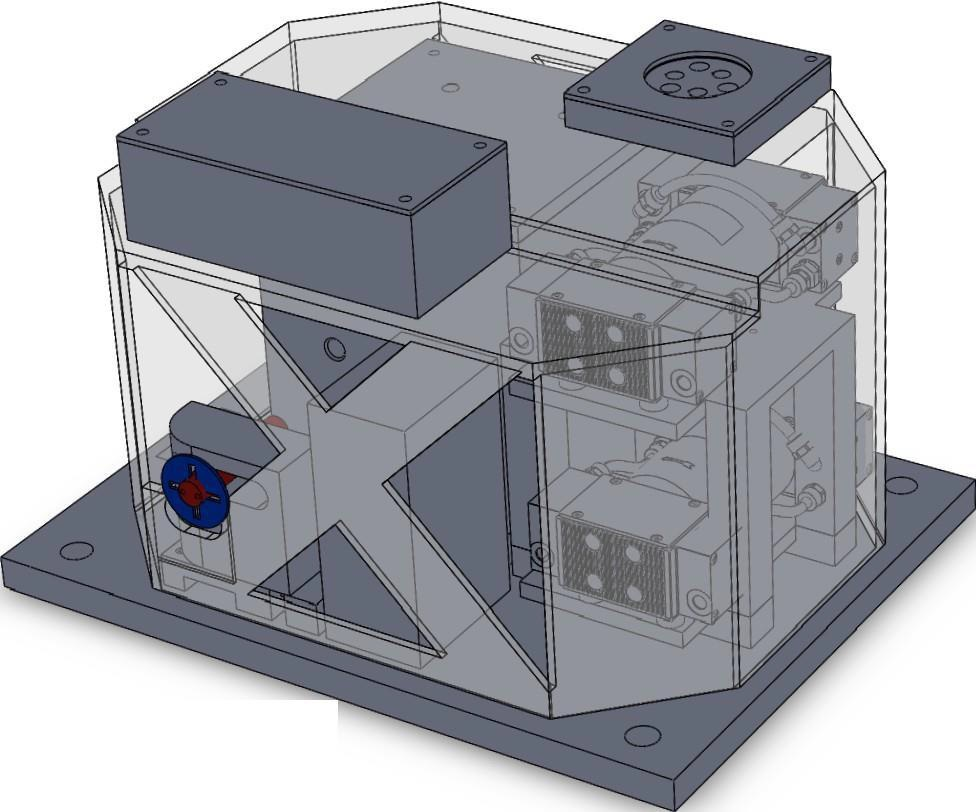
\includegraphics[width=1\textwidth]{./Figures/payload_1.jpg}
\caption{Solidworks design of the SORA payload.}
\label{fig:payload} 
\end{center}
\end{figure}
%Section: Flight Conditions and Environmental Data
\section{Flight}
\label{sec:Flight}
This is the section that could cover the flight details and the environmental data that is not MiniPix.

%\begin{figure}[!htb]
%\begin{center}
%
\includegraphics[width=0.5\textwidth]{./Figures/Test.jpg}
%\caption{This is a test figure.
%}
%\label{fig:Test} 
%\end{center}
%\end{figure}

%
\clearpage
\bibliographystyle{SORA}
\bibliography{SORA}
\end{document}